\section{Scelta dei parametri da ottimizzare}\label{sec:calibrazione}
I pazienti sottoposti a dialisi presentano caratteristiche cliniche anche molto diverse fra loro. Il sesso, l'età, la presenza o meno di comorbidità (diabete, cardiomiopatie, obesità \ldots), e molti altri fattori difficilmente indagabili rendono la risposta alla terapia dialitica molto varia. Per poter adattare il modello allo specifico paziente è necessario quindi usare dei parametri personalizzati. I parametri che si è scelto di ottimizzare sono:
\begin{description}
	\item [$\boldsymbol{\rho}$ :] il coefficiente adimensionale che, all'interno dell'Eq.~(\ref{eq:qfcyes}), regola la permeabilità della membrana capillare, membrana situata fra compartimento plasmatico e interstiziale;
	\item [$\mathbf{k}$ :] il coefficiente di trasferimento di massa ($L/s$) che, all'interno dell'Eq.~(\ref{eq:dmic}), regola per ogni soluto il trasporto diffusivo attraverso la membrana cellulare;
	\item [$\boldsymbol{\eta}$ :] il coefficiente adimensionale che, all'interno dell'Eq.~(\ref{eq:phihdf}), regola per ogni soluto la capacità di estrazione del dializzatore.
\end{description}
\begin{figure}[htbp]
	\centering
		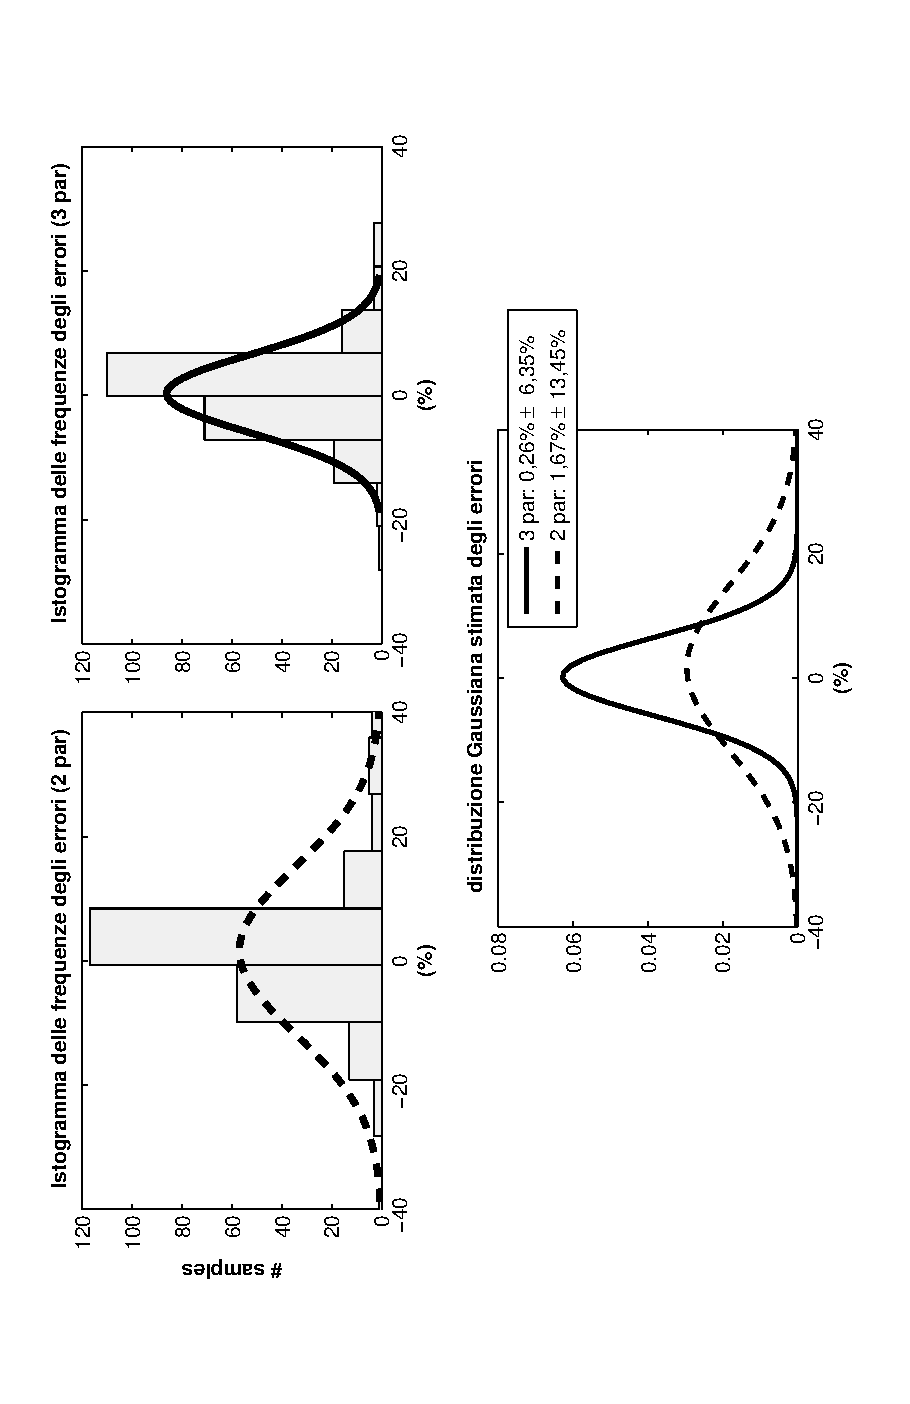
\includegraphics[angle=-90, width=\textwidth]{immagini/2vs3.eps}
	\caption{In alto: confronto fra ottimizzazione a due ($\rho$, $\eta$) e tre parametri ($\rho$,~$k$,~$\eta$). In basso: distribuzione stimata degli errori di simulazione.}
	\label{fig:2vs3}
\end{figure}
Inizialmente si era pensato di calibrare solo i parametri \textbf{$\boldsymbol{\rho}$} e \textbf{$\boldsymbol{\eta}$}, recuperando i valori per il parametro $\mathbf{k}$ da precedenti lavori \cite{casagrande,gatti}. Dopo aver misurato gli errori relativi percentuali fra simulazione e dati clinici di vari pazienti secondo la formula:
\begin{equation}\label{eq:Epercent}
	e_\%(n) = \frac{C_{pl,sim}(n) - C_{pl,cli}(n)}{C_{pl,true}(n)}\cdot 100
\end{equation}
in cui $n$ rappresenta l'$n$-esimo istante di campionamento dei dati ematici per un totale di $225$ misure, e i pedici \textit{sim} e \textit{true} indicano rispettivamente misure provenienti dalla simulazione numerica e dalla realtà clinica, si è fatto il confronto tra la distribuzione degli errori che si commettono quando si calibrano solo due paramtri rispetto a quando invece se ne calibrano tre. In \figurename~\ref{fig:2vs3} sono mostrati gli istogrammi delle frequenze di tali errori (due parametri in alto a sinistra; tre parametri in alto a destra). Nella stessa figura, in basso, è mostrata la stima gaussiana di tali errori\footnote{il test di Shapiro-Wilk conferma, con un p-value inferiore a $0,001$, la gaussianità delle due distribuzioni.}, dalla quale si riscontra che con la calibrazione a tre parametri gli errori, sebbene ci sia qualche \textit{outlier}, si riducono rientrando nella fascia $\pm 20\%$.
